The scenarios- and implementation of the workshop.

\section*{Introduction (10min)}
We are studying the fifth year at computer science program at LTU and for now doing our project. As a part of our prestudy are we hosting this workshop where we will investigate possibilities through a couple of scenarios. You will do a couple of assignments in groups and then present your result and discuss these with others.

\section*{Scenario 1 (10 min + 10 min discussion)}
You have just started a course where you will learn to program in a language you don't find interesting. The teacher has given you lot recommended assignments but non seems interesting. Which type of system or moments would motivate you to do the assignments. Dream free.
\begin{itemize}
\item Which subject do you think has this problem?
\item Do the assignment needs to be presented? If so how?
\item Which material is needed?
\item What should be on a list with highlights?
\end{itemize} 

\section*{Scenario 2 (10 min + 10 min discussion)}
After many years you are the teacher for that boring course. The boss comes in to your office a Friday afternoon and says that the course moments are to few and you need to update them till Monday. You sits down as the motivated teacher you are and thinks about a system than would motivate students, you remember your old concept.

You want to make this work for a long time, which limitations must you as a teacher do?
\begin{itemize}
\item What is most time consuming?
\item Is it possible to sort your highlight after time consuming?
\item How long time can the moment take to develop and maintain?
\end{itemize} 

\section*{Scenario 3 15 min + 10 min discussion}
Now when you have a working system and it scales along the new courses you teach in, but the students wants a e-tool. How does this tool look like?, Think web besides details and try to catch the users experience.

\begin{itemize}
\item How do you do inputs?
\item How does your highlights look like practical?
\item Do you see any limitations?
\end{itemize} 


\section*{Results}
\subsection*{Scenario 1}
\begin{itemize}
\item Let assignments interlink.
\item Be able to choose which assignments should be done.
    \begin{itemize}
    \item Hard to grade, every goal of the course need to be met.
    \item Assignments with similar content.
    \end{itemize}
\item Constructive alignment, how goals, assignments and examination interacts.
\item Early and quick feedback.
\item Formative assessment, continuous feedback.
\item Groups assignments, hide the personal result.
\item AI Avatar that gives feedback.
\item Lot of visualization of the result.
\item Present the purpose of the assignment.
\item Different angle of the design depending on the user which is solving the assignment.
\end{itemize}

\subsection*{Scenario 2}
\begin{itemize}
\item Not everything in a course should be change at same time.
\begin{itemize}
\item Old assignments could be divided.
\item Shorter feedback loop.
\item old assignments with new context.
\end{itemize}
\item Updating the course introduction is cheap and makes the goals of the course more clear.
\item When the knowledge should be tested.
\begin{itemize}
\item Thoroughly, min/max, median or average.
\item In the end there is a written exam.
\end{itemize}
\item Invoke from elder students.
\item Peer-to-peer feedback.
\item Test one implementation even if it's bad.
\item Students create assignments for each other.
\end{itemize}

\subsection*{Scenario 3}
\begin{itemize}
\item Anonymous questions live
\begin{itemize}
\item ``Did you understand what I said?''
\item Direct feedback.
\end{itemize}
\item Direct chat, students and teacher.
\item Auto generated feedback to the teacher.
\begin{itemize}
\item Aggregate data from relevant measurements.
\end{itemize}
\item A student knowledge bank.
\begin{itemize}
\item Wiki.
\end{itemize}
\item Code correction / evaluation.
\end{itemize}

\subsection*{Photos}
\begin{figure}[H]
\centering
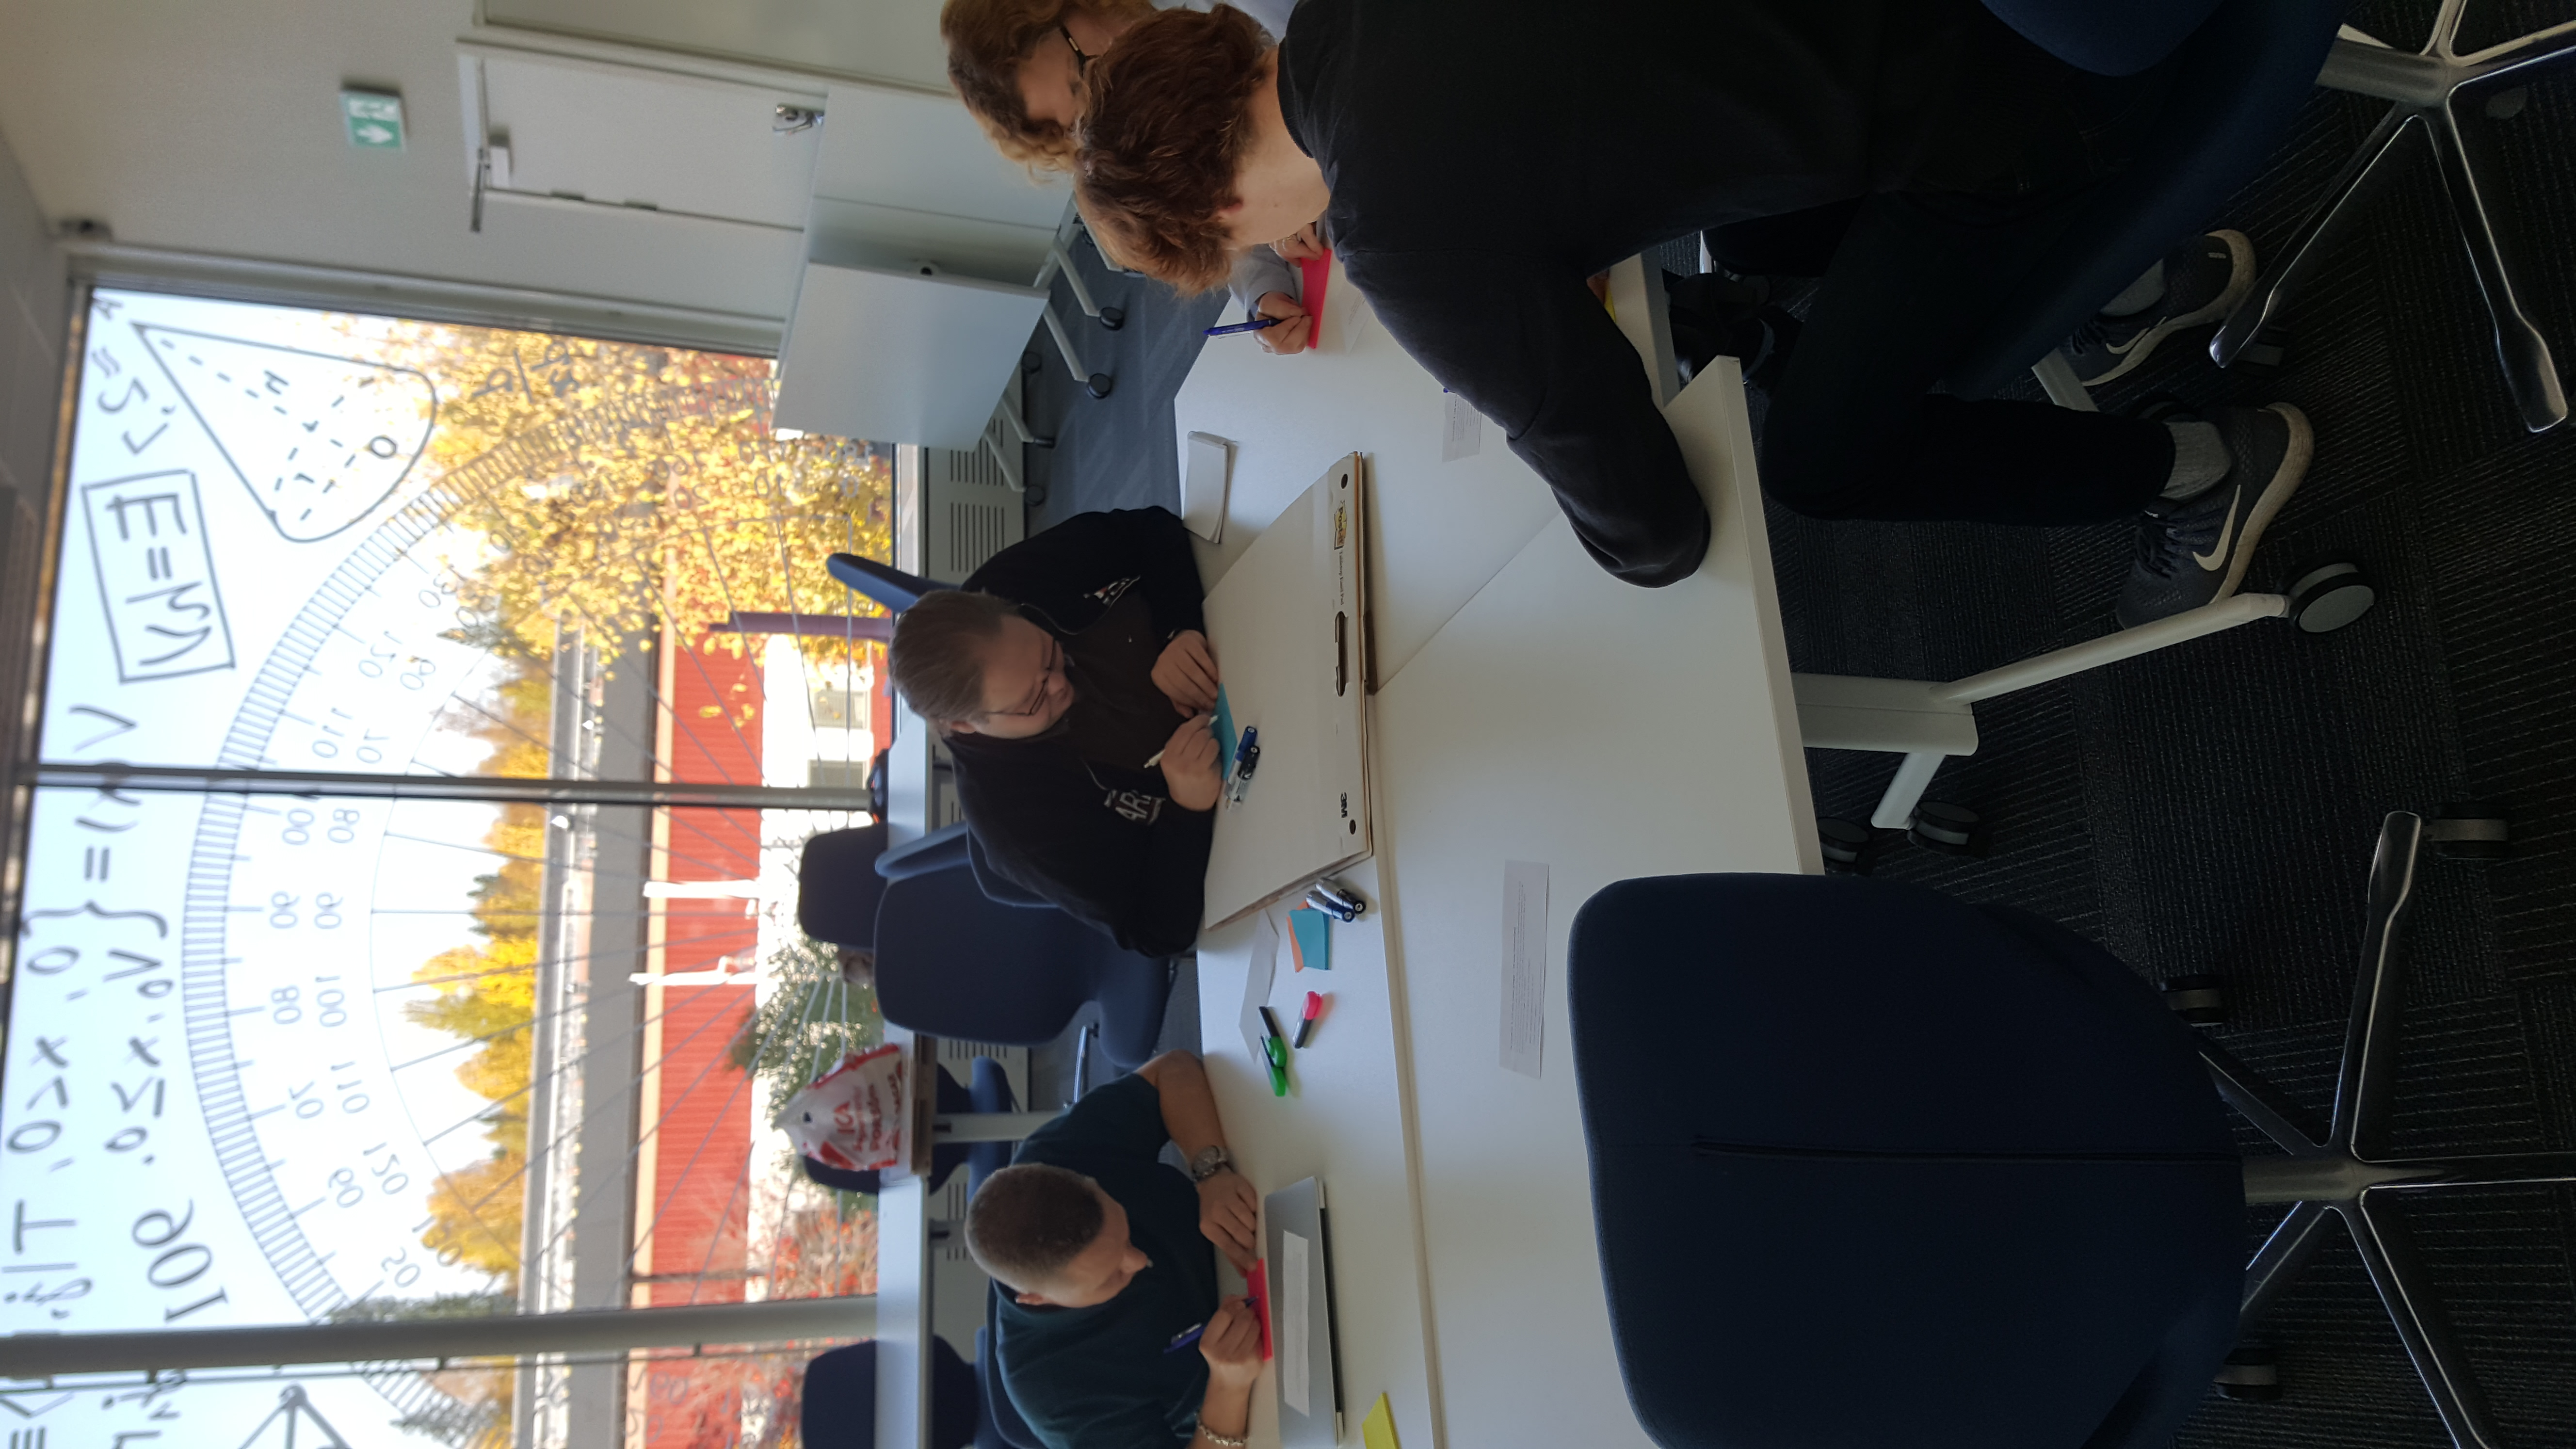
\includegraphics[width=0.8\textwidth]{img/workshop1.jpg}
\caption{Workshop}
\label{fig:workshop1}
\end{figure}

\begin{figure}[H]
\centering
\includegraphics[width=0.8\textwidth]{img/workshop2.jpg}
\caption{Workshop}
\label{fig:workshop2}
\end{figure}

\begin{figure}[H]
\centering
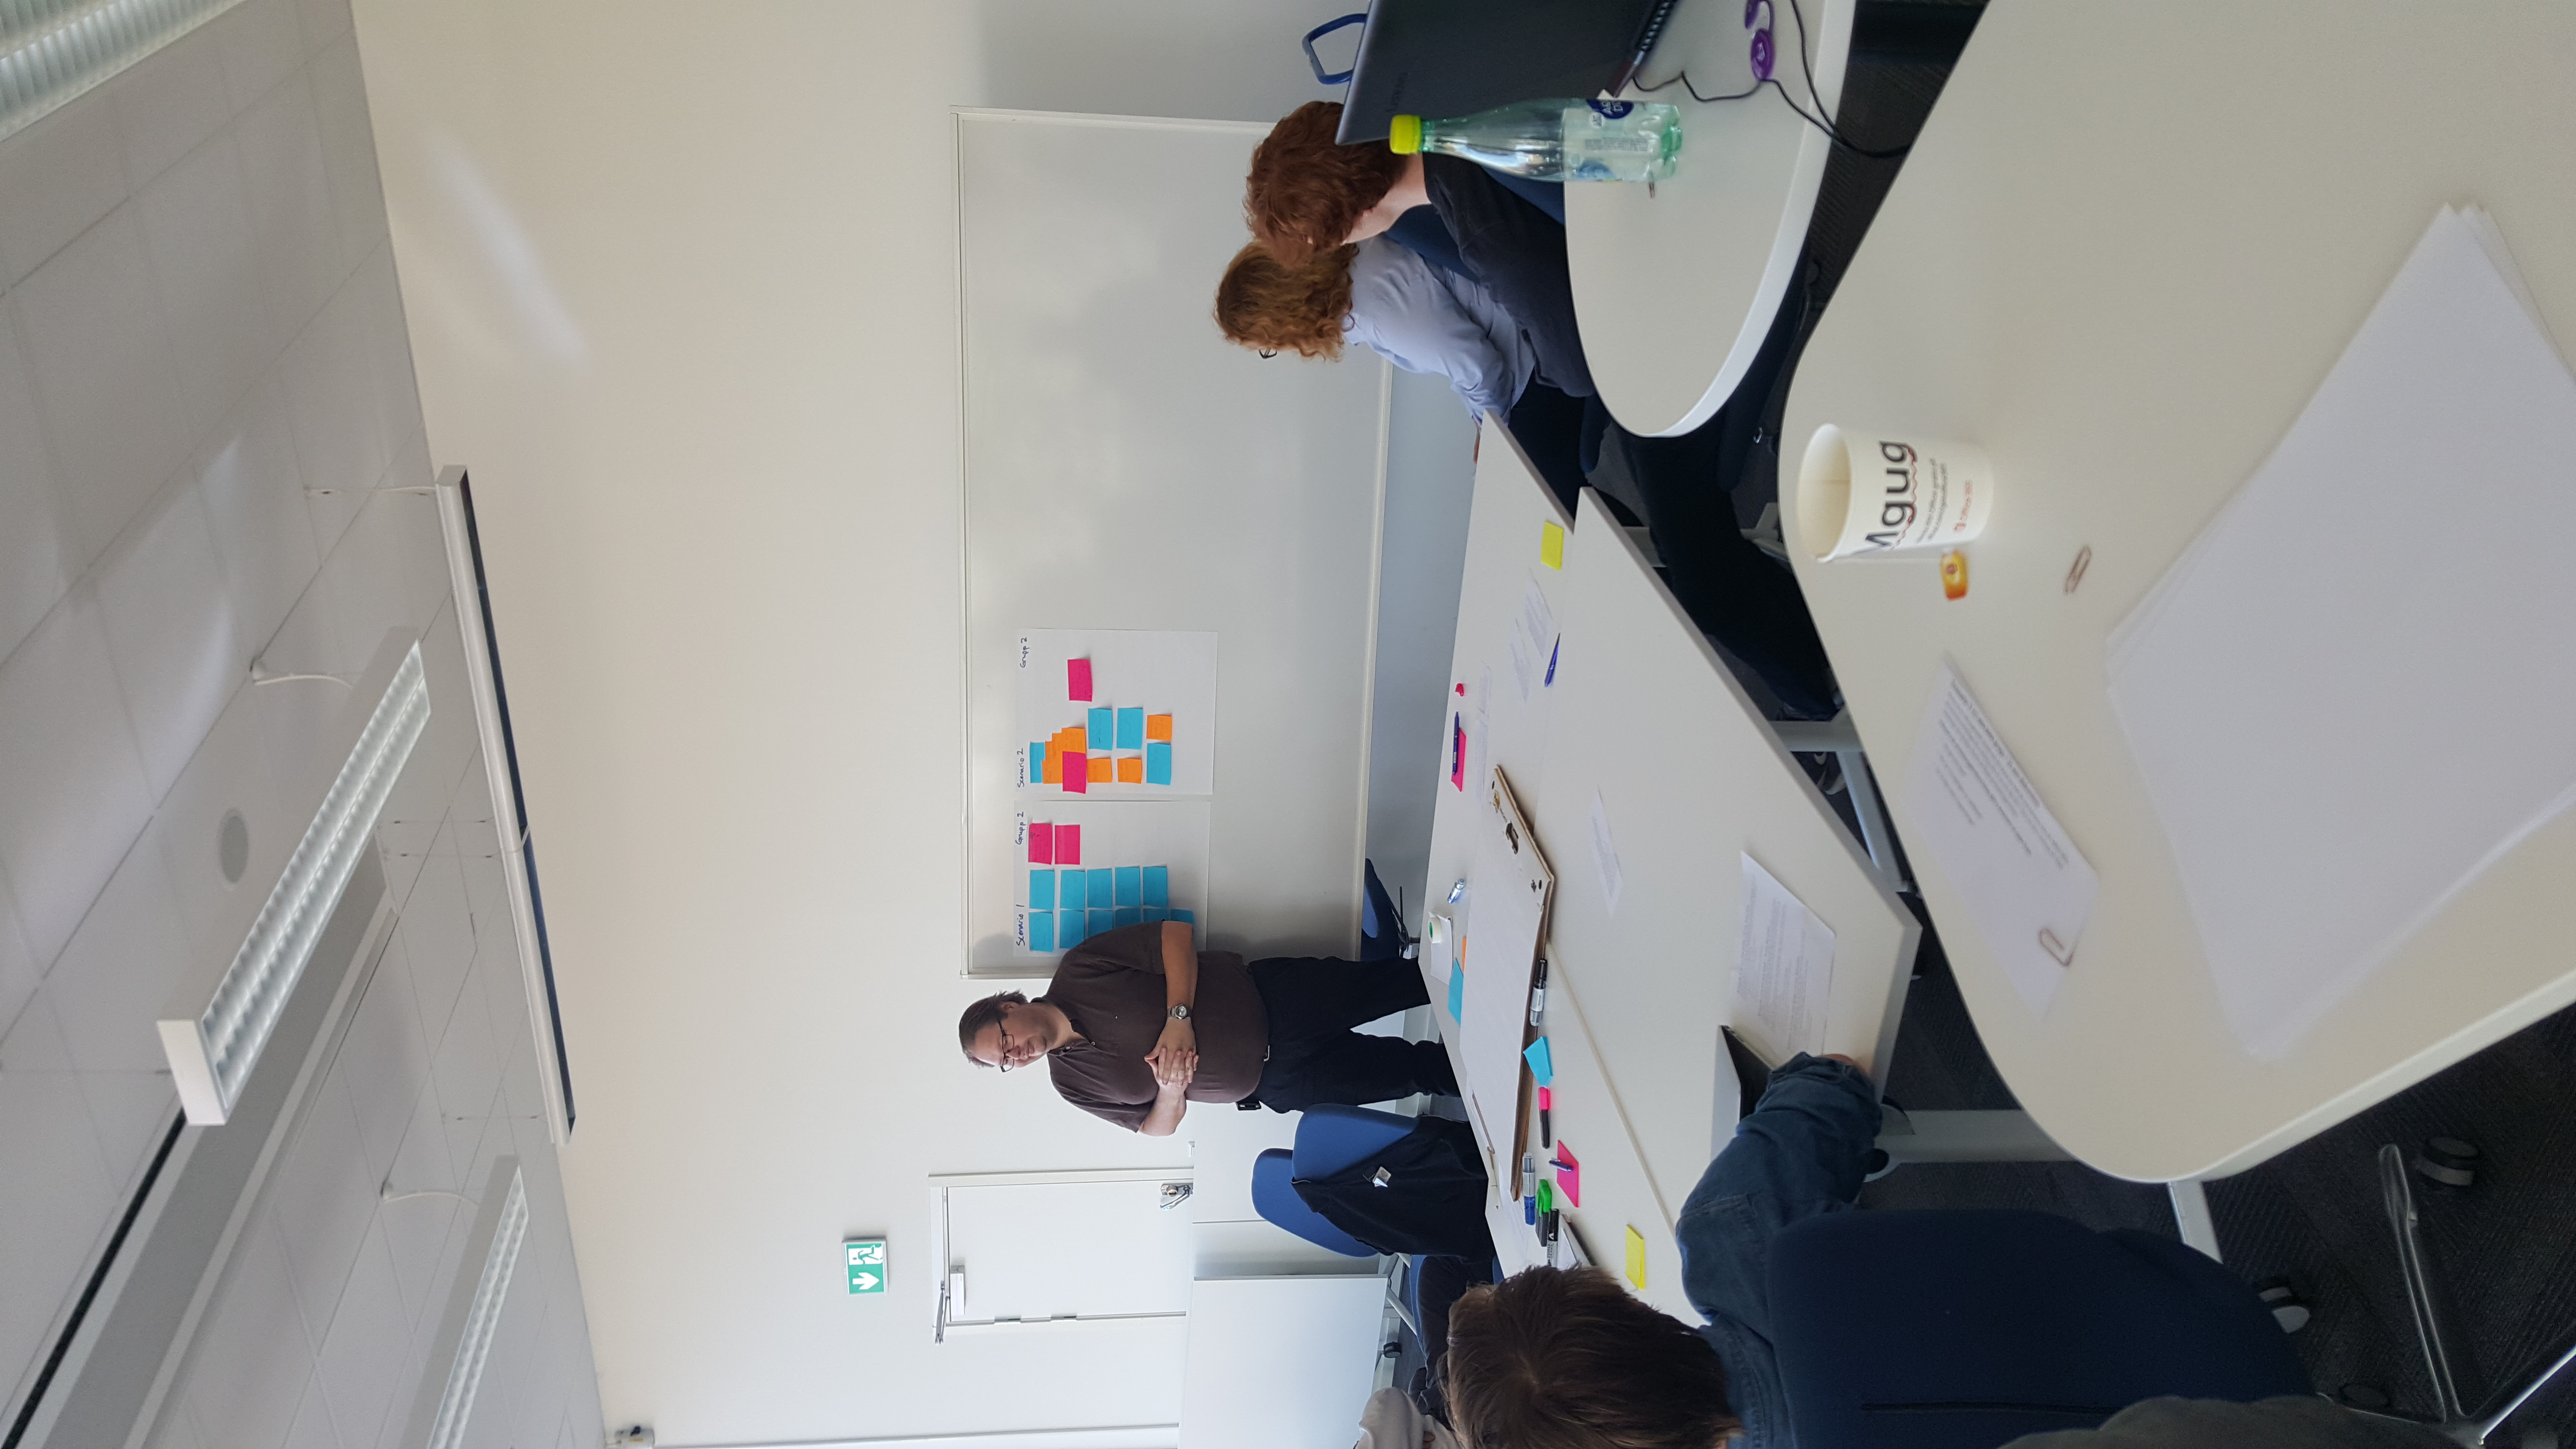
\includegraphics[width=0.8\textwidth]{img/workshop3.jpg}
\caption{Workshop}
\label{fig:workshop3}
\end{figure}
